\documentclass{beamer}

\usepackage{beamer_tom}
\graphicspath{{./images/}}
\def\TikzLocation{./tikz/}
\def\tkzscl{1}

\def\biblio{
	\nobibliography{../../library}
	\def\biblio{}
}

\institute{INRIA Saclay}
\author{Thomas Moreau}
\title{
	Learning step sizes for\\unfolded sparse coding}

\date{
	May 29, 2018
}

\collaborators{Pierre Ablin; Mathurin Massias; Alexandre Gramfort}

\setbeamertemplate{title page}[frame]
\def\extraLogo{}
\DeclareMathOperator*{\supp}{Supp}

\begin{document}
	
	\begin{frame}
		\titlepage
		\biblio{}
	\end{frame}

\begin{frame}{Electrophysiology}
\begin{columns}[c]
    \column{.5\textwidth}
    \textbf{Magnetoencephalography}\\
    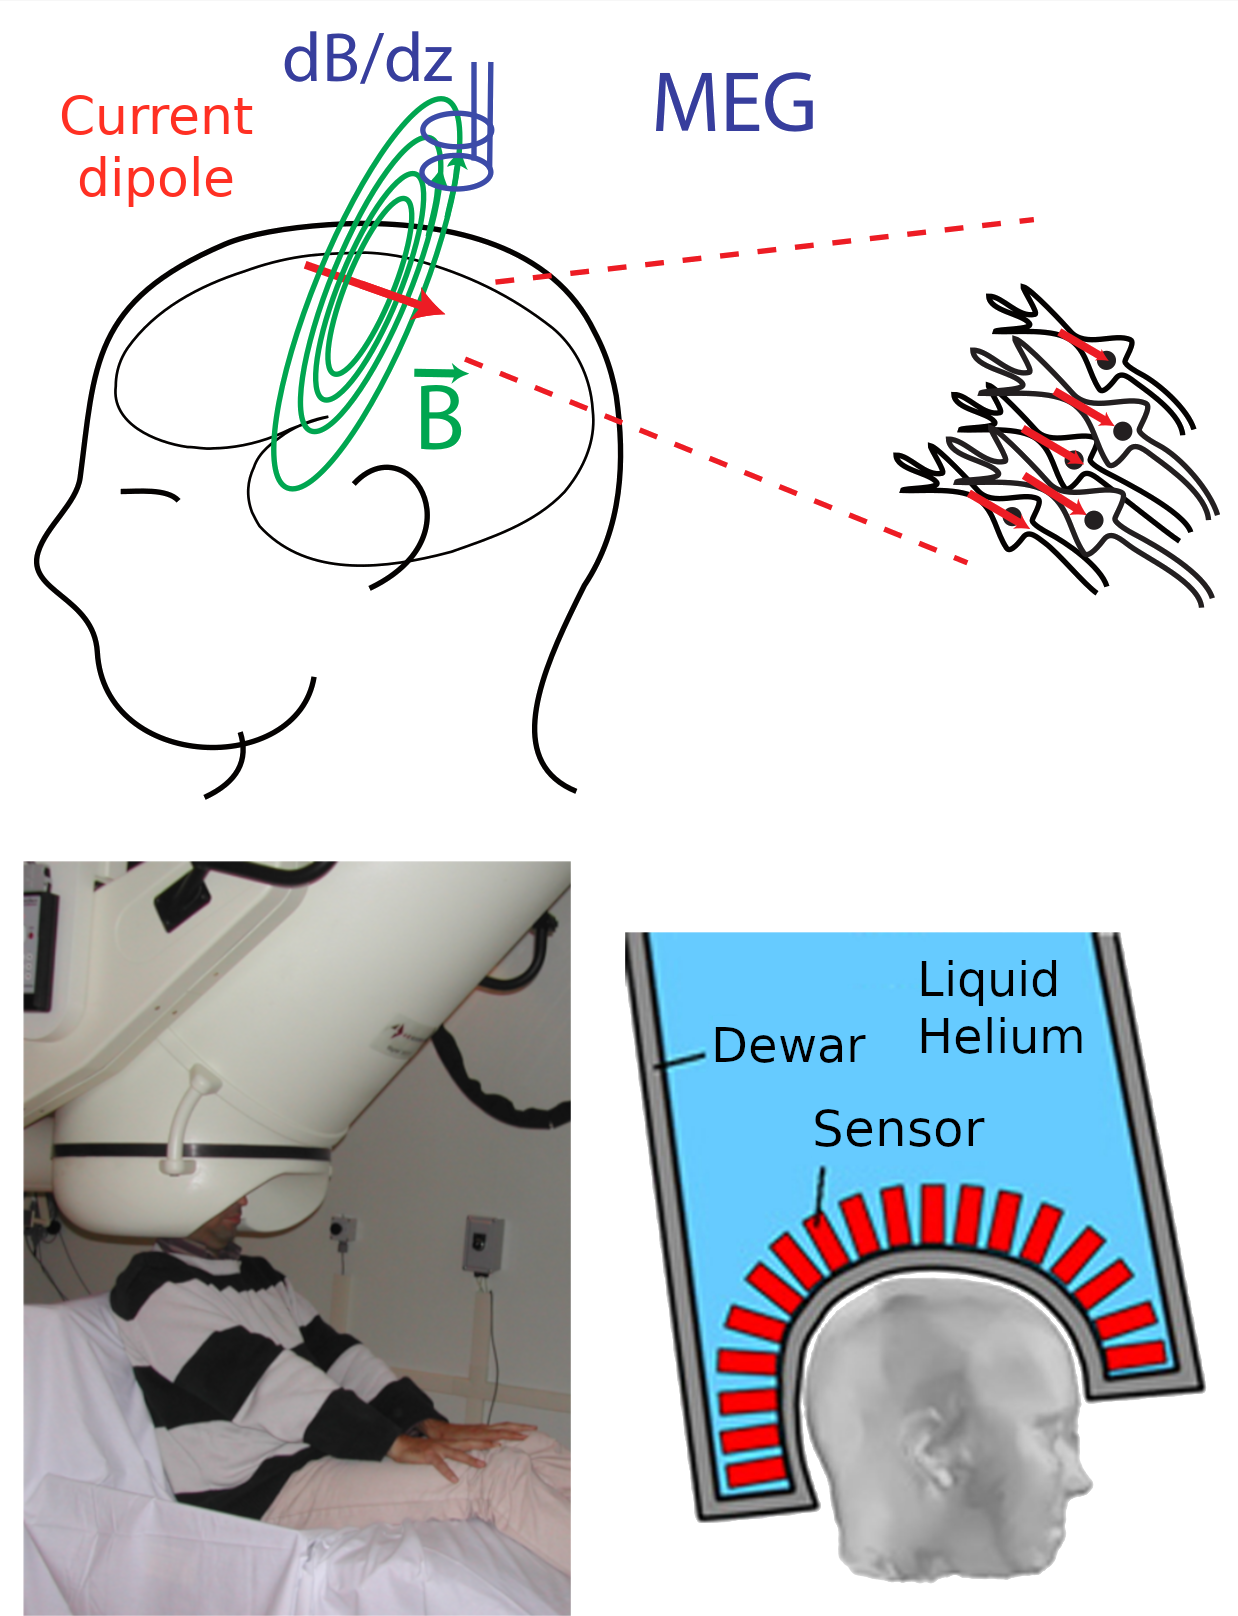
\includegraphics[width=.8\linewidth]{meg_presentation}
    \column{.5\textwidth}
    \textbf{Electroencephalography}\\
    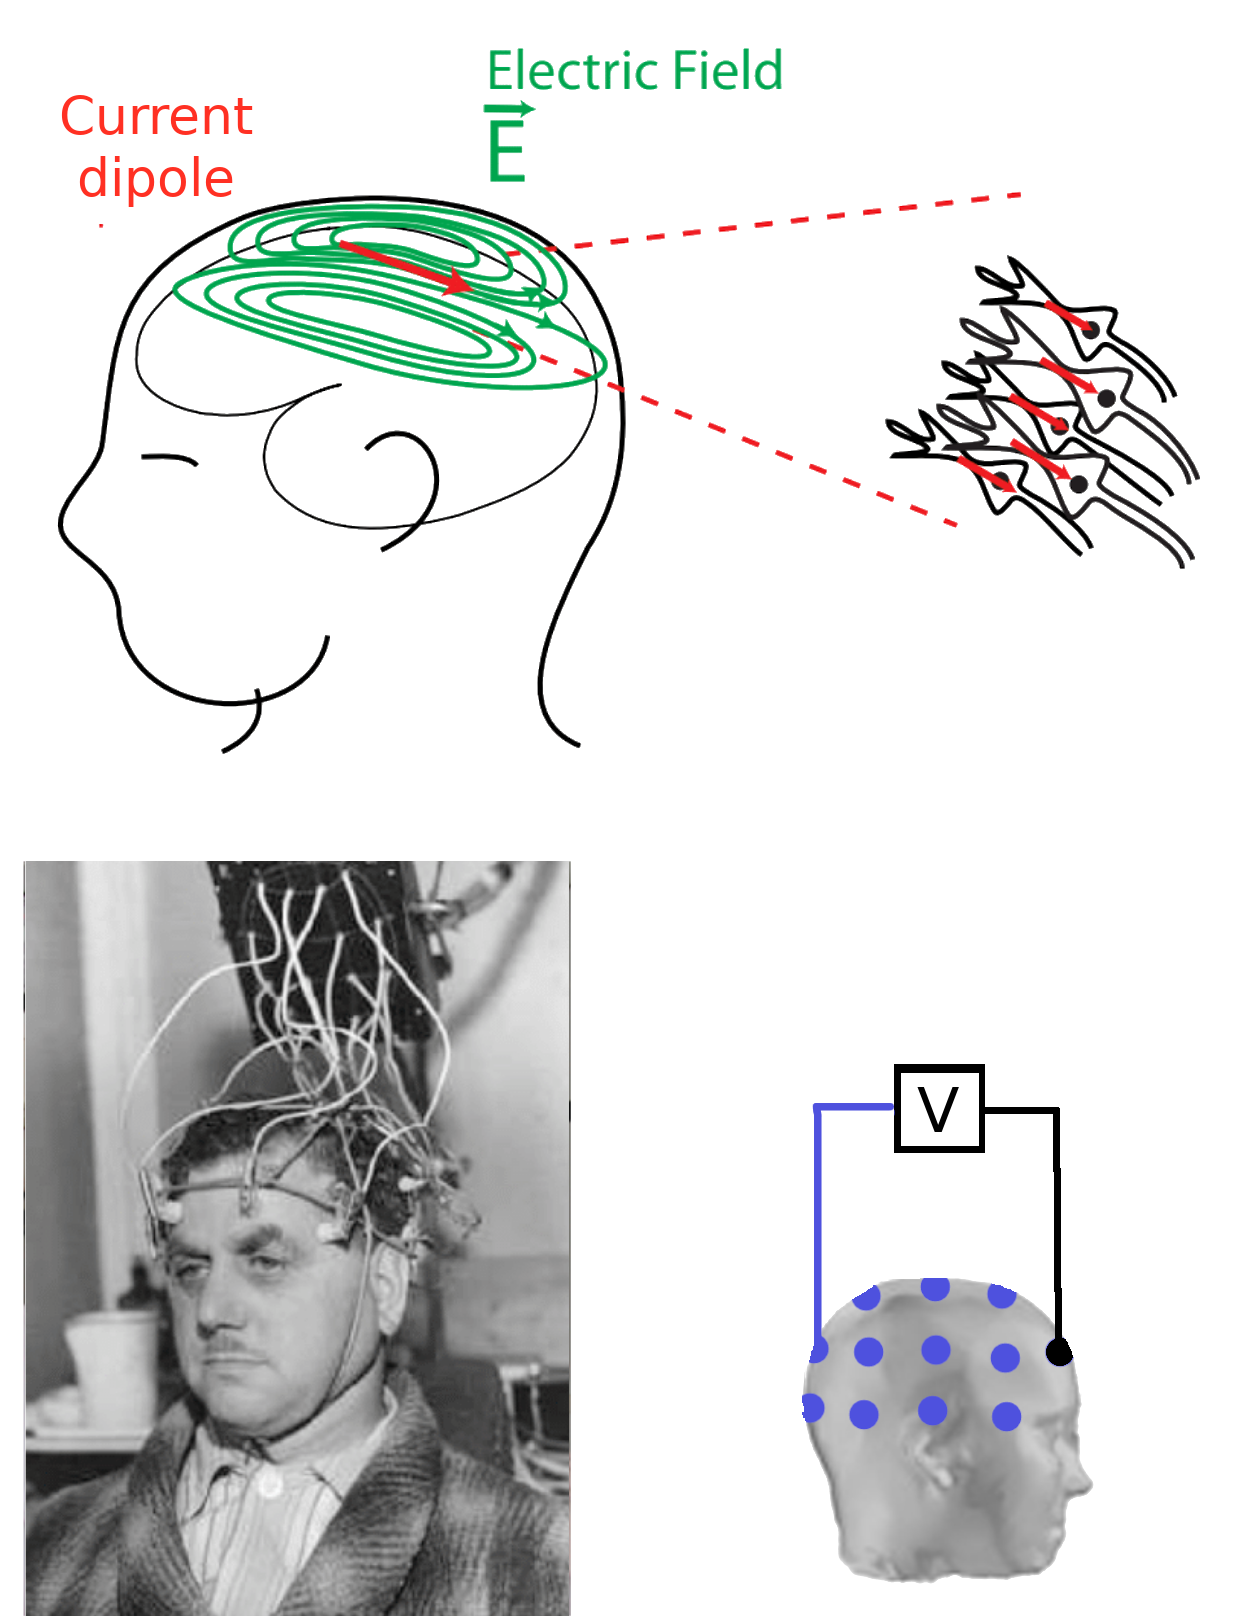
\includegraphics[width=.8\linewidth]{eeg_presentation}
\end{columns}
\end{frame}
	
	\begin{frame}{Inverse problems}
		
        \definecolor{Z}{RGB}{45,162,65}
        \definecolor{D}{RGB}{180,35,35}
        \def\varX{{\color{linkcolor} \pmb x}}
        \def\varZ{{\color{Z} \pmb z}}
        \def\varD{{\color{D} \pmb D}}
        {\centering
        \begin{tikzpicture}
        \tikzset{
            %Define standard arrow tip
            >=stealth',
            %Define style for boxes
            varstyle/.style={
                rectangle,
                rounded corners,
                draw=black,
                text width=1em,
                minimum height=1.5em,
                text centered},
        }
        \node (meg) {
            \alt<3->{%
                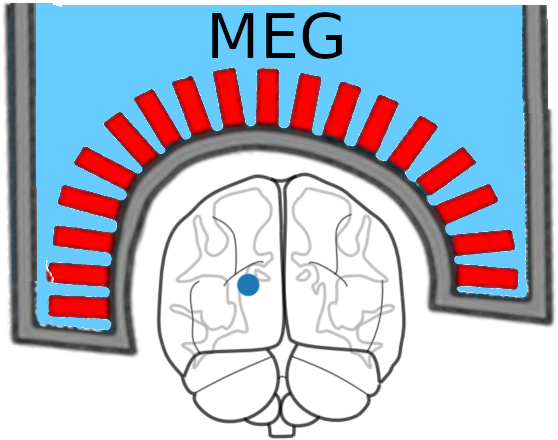
\includegraphics[width=12em]{meg_localised_source}
            }{%
                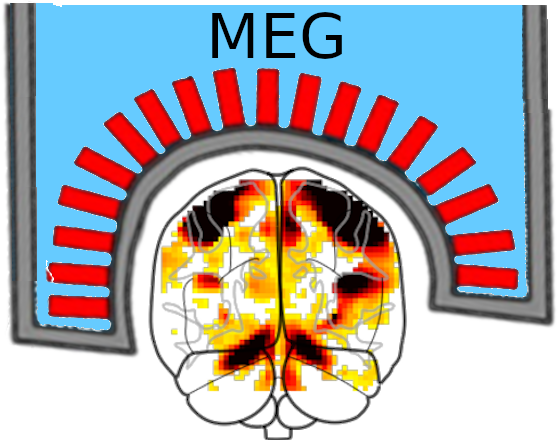
\includegraphics[width=12em]{meg_source}
            }};
        \draw[->, thick] ($(meg.east) - (0, 1.5em)$) -- ++(8em, 0)
        node[midway, align=center] (maxwell) {Maxwell's\\Equations}
        node[right] (topomap) {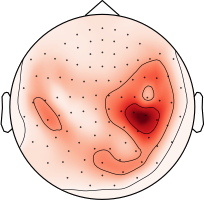
\includegraphics[width=6em]{topomap_somato}};
        \node[varstyle, below=.5em] at (topomap.south) (varX) {$\varX$};
        \node[below=0em of varX.south] {\bf Observed signal};
%        \draw[->, thick] (topomap.east) -- ++(5em, 0)
%        node[midway, align=center] {\small Problème\\ \small inverse}
        \node[varstyle, below=.2em of meg]
            (varZ) {$\varZ$};
            \node[below=0em of varZ.south] {\bf Electrical activity};
        \node[varstyle, below=3.8em of maxwell.center]
            (varD) {$\varD$};
            
        \uncover<2->{
             \draw[<-, thick] (meg.east) to[bend left, looseness=1]
                node [midway, above] {Inverse Problem}
                ($(topomap.west) + (0, 1.5em)$);
        }
        \end{tikzpicture}}
        \vskip0em
        {\bf Forward model: }$\varX{} = \varD\varZ$
        \hskip3em
        \uncover<2->{{\bf Inverse problem:} ill-posed}\\[1em]
        \uncover<3->{\centering
               Optimization with a regularization $\mathcal R$ encoding prior knowledge\\ $\argmin_{\varZ} \|\varX{}
        - \varD{}\varZ{}\|_2^2 + \mathcal R(\varZ{})$\\[1em]
               Example: sparsity with $\mathcal R = \lambda\|\cdot\|_1$}

	\end{frame}

\begin{frame}{Inverse problem: Other domains}

    
\begin{columns}[T]
    
    \column{.5\textwidth} {\bf Ultra sound}\\
    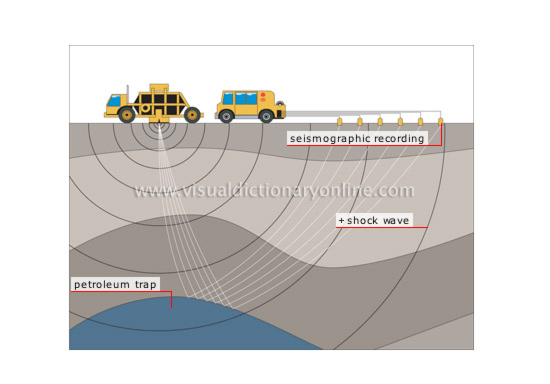
\includegraphics[width=.7\textwidth, trim={6.7em 4em 7em 5em}, clip]{InverseProblem_petroleum}

    \column{.5\textwidth}{\bf fMRI - compress sensing}\\
        \begin{columns}[c]
        \column{.5\textwidth}    \centering
        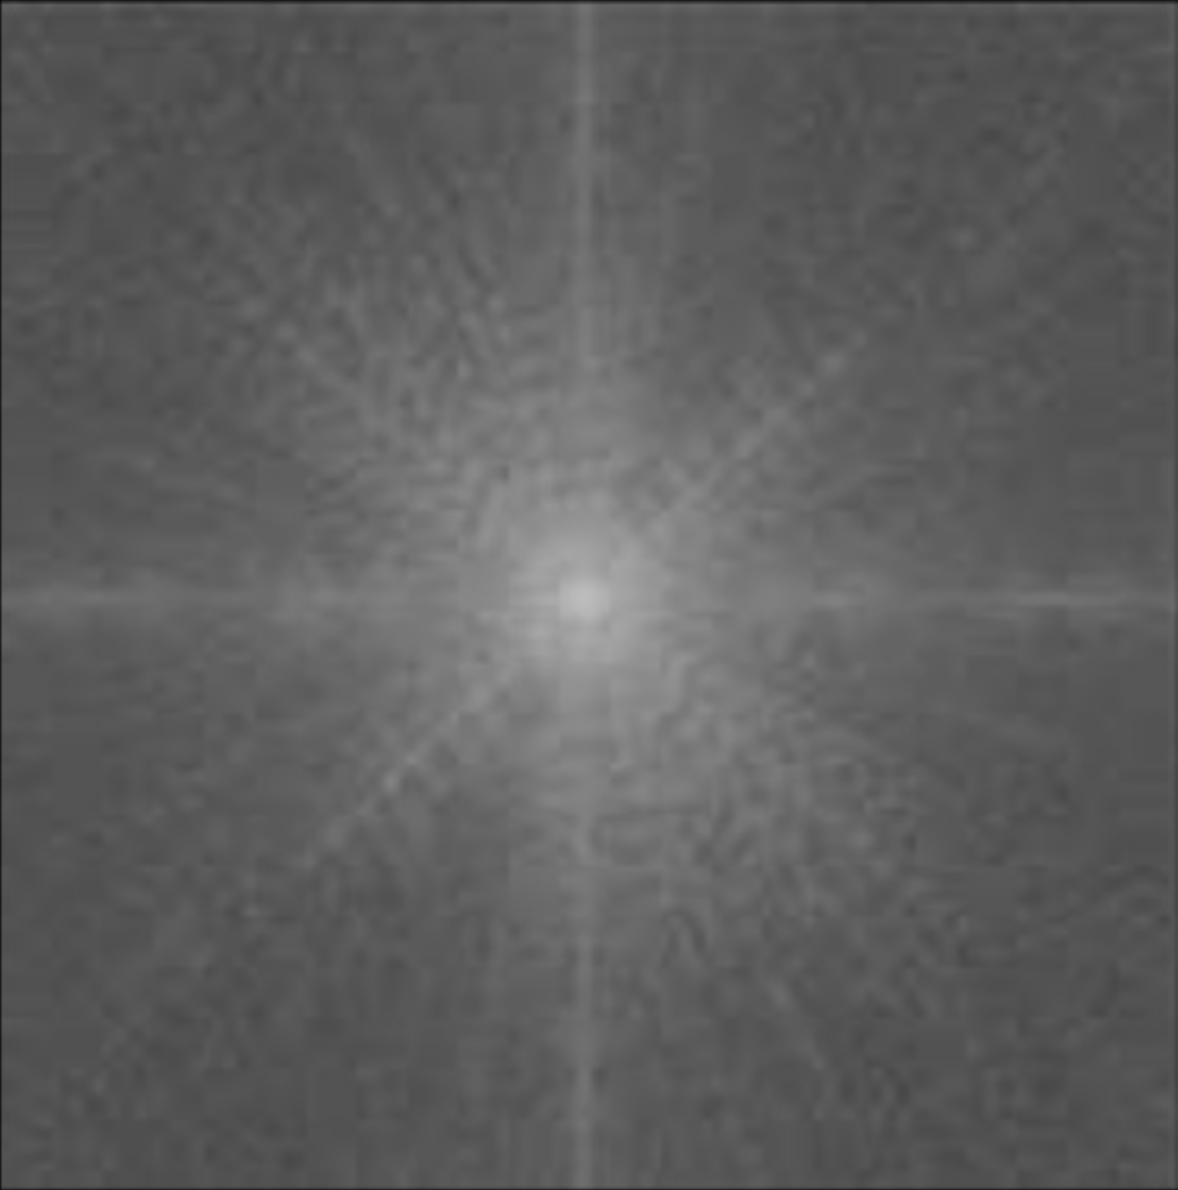
\includegraphics[width=.8\textwidth]{K_space}\\
        \column{.5\textwidth} \centering
        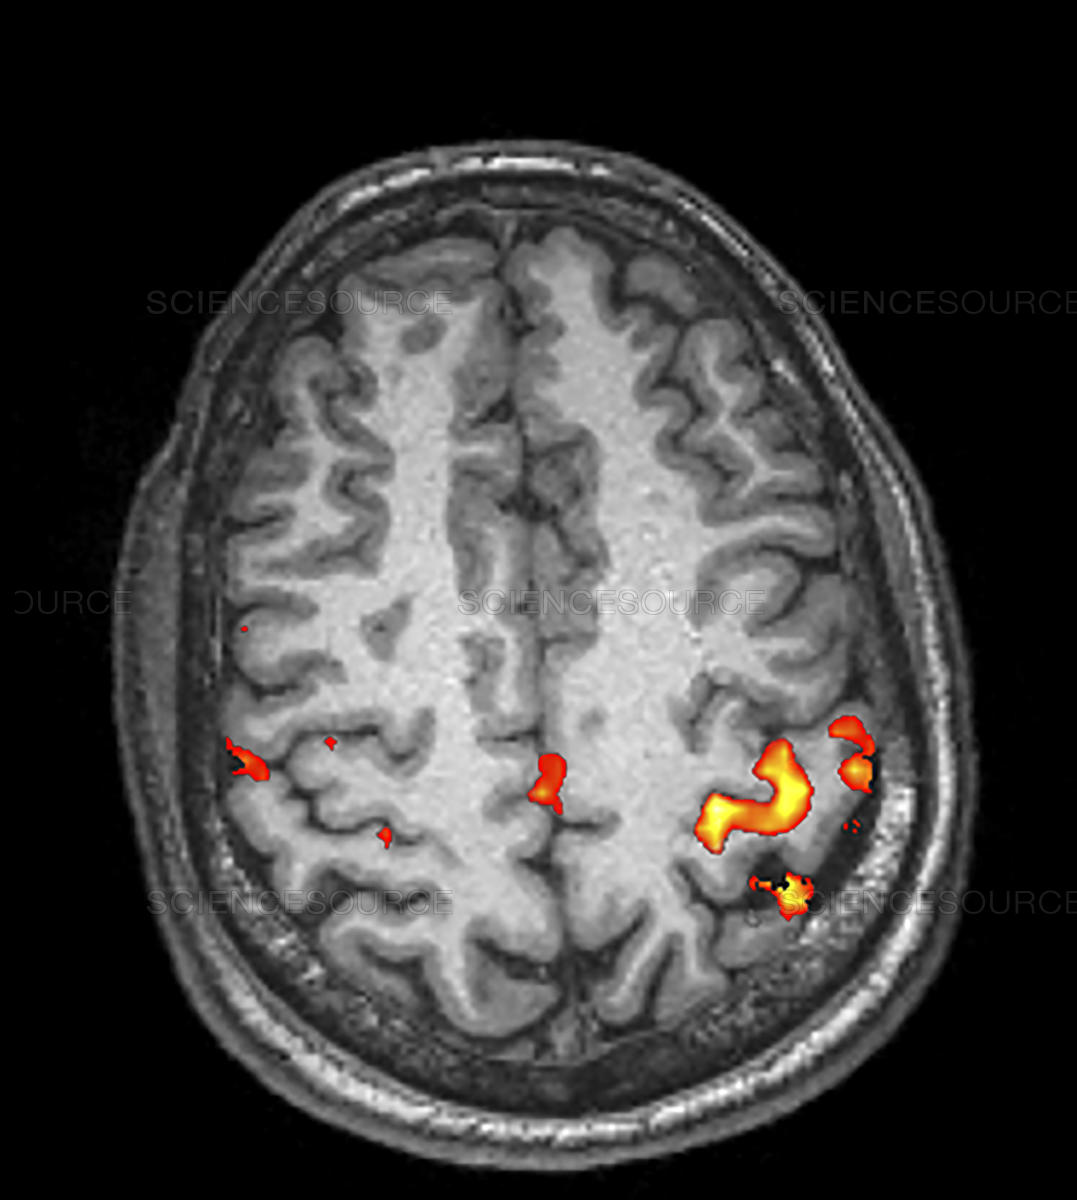
\includegraphics[width=.8\textwidth]{brain_scan}\\
        \end{columns}
    \end{columns}
    \vskip1em
    {\bf Astrophysic}\\
    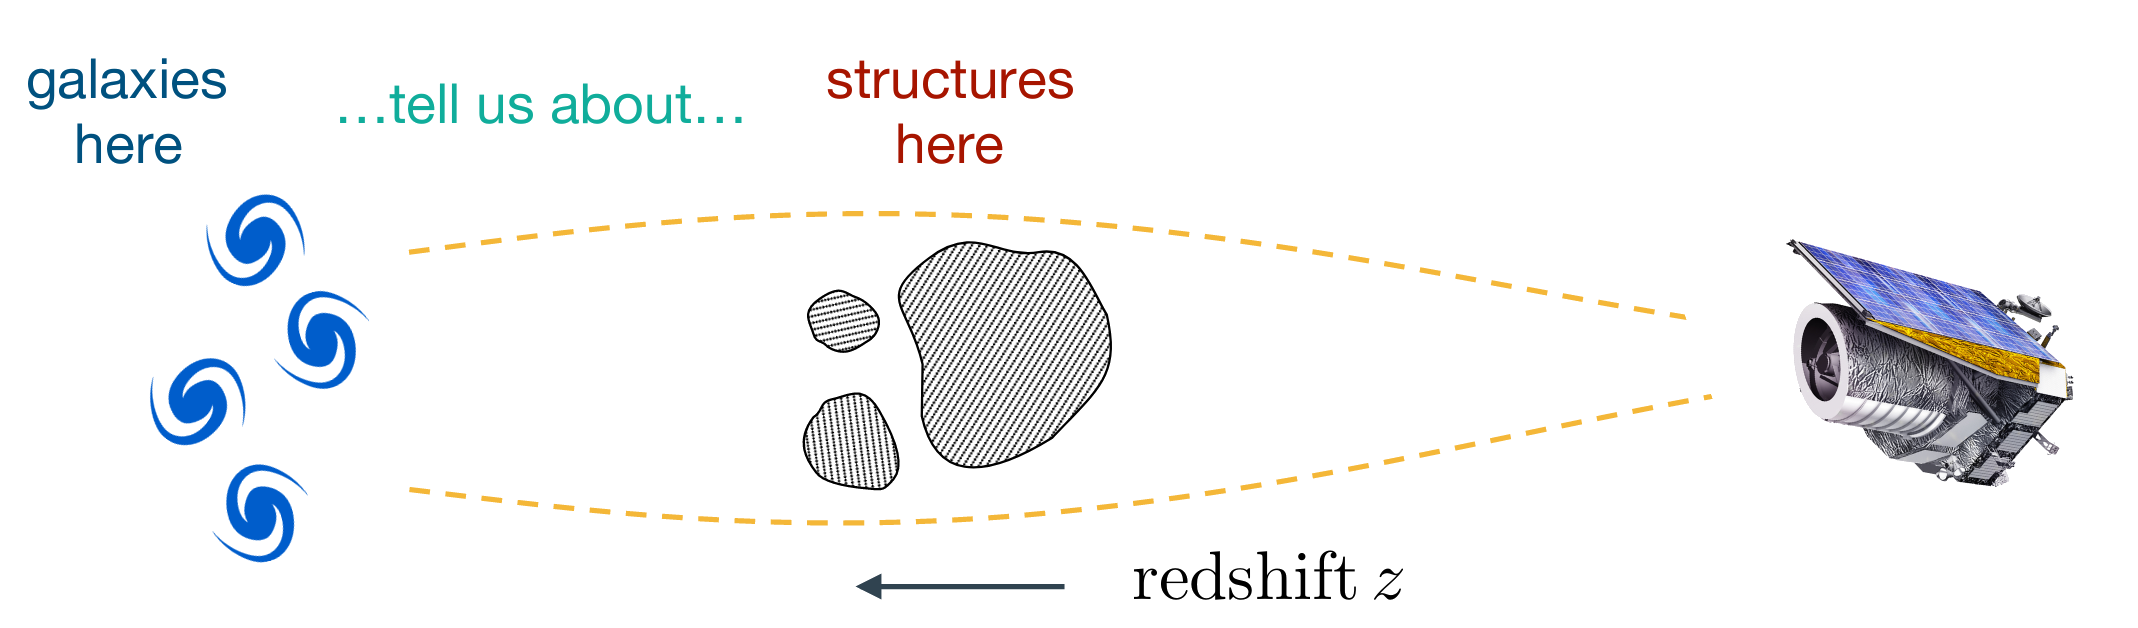
\includegraphics[width=\textwidth]{weak_lensing}

\end{frame}

\begin{frame}{Some challenges for inverse problems}


    \setlength\bodywd{.9\linewidth}
    \centering
    \highlight[wd=\bodywd, c=black]{\raggedright\textcolor{darkred}{\bf Evaluation:}
    \normalfont often there is no ground truth,\\[0em]
    \begin{itemize}\color{black}\itemsep0em
        \item[$\bullet$] In neuroscience, we cannot access the brain electrical activity.%
        \item[$\bullet$] How to evaluate how well it is reconstructed?\\
        \keypoint{Part of my research topic}
    \end{itemize}%
    }\vskip.5em
    %
    \highlight[wd=\bodywd, c=black]{\raggedright\textcolor{darkred}{\bf Modelization:}
    \normalfont how to better account for the image structure,\\[0em]
    \begin{itemize}\color{black}\itemsep0em
        \item[$\bullet$] $\ell_2$ reconstruction evaluation does not account for localization%
        \item[$\bullet$] Optimal transport could help in this case?\\
        \keypoint{Hicham and Quentin projects}
    \end{itemize}%
    }\vskip.5em
    %
    \highlight[wd=\bodywd, c=black]{\raggedright\textcolor{darkred}{\bf Computational:}
        \normalfont solving these problems can be too long,\\[0em]
        \begin{itemize}\color{black}\itemsep0em
            \item[$\bullet$] Many problems share the same forward operator $\pmb D$%
            \item[$\bullet$] Can we use the structure of the problem?\\
            \keypoint{Today talk topic!}
        \end{itemize}%
    }\vskip.5em
    %
\end{frame}

\section{Better step sizes for\\Iterative Shrinkage-Thresholding Algorithm (ISTA)}
\parttitleframe{}

\begin{frame}{Sparse Coding}

    For a dictionary $D \in \Rset^{n\times m}$ and $\lambda > 0$, sparse coding for $x\in \Rset^n$ is \\[.5em]
    \[
    z^{*} = \argmin_{z} F_x(z) = 
    \underbrace{\frac{1}{2}\| x - D z\|_2^2}_{f_x(z)}
    + \lambda\| z\|_1
    \]
    \emph{a.k.a.} Lasso, sparse linear regression, ...\\[1em]
    We are interested in the case where $m > n~.$\\[2em]
    {\centering
    \setlength\bodywd{.9\linewidth}
    \begin{block}{\bf Properties}
        \begin{itemize}\color{black}\itemsep.5em
            \item The problem is convex in $z$ but not strongly convex in general
            \item $z=0$ is solution if and only if
                $\lambda \ge \lambda_{\max} \doteq \|D^\top x\|_\infty$
        \end{itemize}
    \end{block}}
\end{frame}

\begin{frame}{Iterative Shrinkage-Thresholding Algorithm \mycite{Daubechies2004}}
    Proximal gradient descent algorithm
    \[
        z^{(t+1)} = \text{ST}\left(z^{(t)}
                                   - \frac{1}{L}\underbrace{\nabla f_x(z^{(t)})}_{D^\top(D z^{(t)} - x)},
                                   \frac{\lambda}{L}\right)
    \]
    where $L = \|D^\top D\|_2$ is the largest eigen-value of $D^\top D$.\\
    Here, $1/L$ play the role of a step size.
    \begin{block}{Convergence rates}
       If $f_x$ is $\mu$-strongly convex, \ie{} $\sigma_{\min}(D^TD) \ge \mu > 0$
       \[
            F_x(z^{(t)}) - F_x(z^*) \le \left(1 - \frac{\mu}{L}\right)^t\left(F_x(0) - F_x(z^*)\right)
       \]
       In the general case, $F_x(z^{(t)}) - F_x(z^*) \le \frac{L\|z^*\|_2}{t}$\\
     \end{block}
\end{frame}

\begin{frame}[t]{ISTA: Majoration-Minimization}
    Taylor expansion of $f_x$ in $z^{(t)}$
    \begin{align*}
        F_x(z) &  = f_x(z^{(t)}) + \nabla f_x(z^{(t)})^\top(z - z^{(t)}) + \lambda\|z\|_1\\
               & \hskip10ex + \frac{1}{2}(z - z^{(t)})D^\top D(z - z^{(t)})\\
               & \le f_x(z^{(t)}) + \nabla f_x(z^{(t)})^\top(z - z^{(t)}) + \frac{L}{2}\|z - z^{(t)}\|_2^2 + \lambda\|z\|_1
    \end{align*}
    Replace the Hessian $D^\top D$ by $L \textbf{ Id}$.\\[2em]
    
    Separable function that can be minimized in close form
    \begin{align*}
        \argmin_z \frac{L}{2}\left\|z^{(t)} - \frac{1}{L}\nabla f_x(z^{(t)}) - z\right\|_2^2 + \lambda\|z\|_1
        & = \text{ST}\left(z^{(t)} - \frac{1}{L}\nabla f_x(z^{(t)}),
                           \frac{\lambda}{L}\right)\\
        & = \text{prox}_{\frac{\lambda}{L}}\left(z^{(t)} - \frac{1}{L}\nabla f_x(z^{(t)})\right)
    \end{align*}
\end{frame}

\begin{frame}{ISTA: Majoration for the data-fit}
    \definecolor{darkgreen}{RGB}{0, 148, 0}
    \myitem{} Hessian $D^\top D
                       \only<2>{\prec \color{red} L \textbf{ Id}}
                       \only<3>{\prec \color{blue} A^\top \Lambda A}
                       \only<4>{\prec \color{darkgreen} L_S \textbf{ Id}}$
              \only<3>{\mycite{Moreau2017}}
              \only<4>{on support $S$}\\
    \centering
    \makebox[.75\textwidth][c]{
        \only<1>{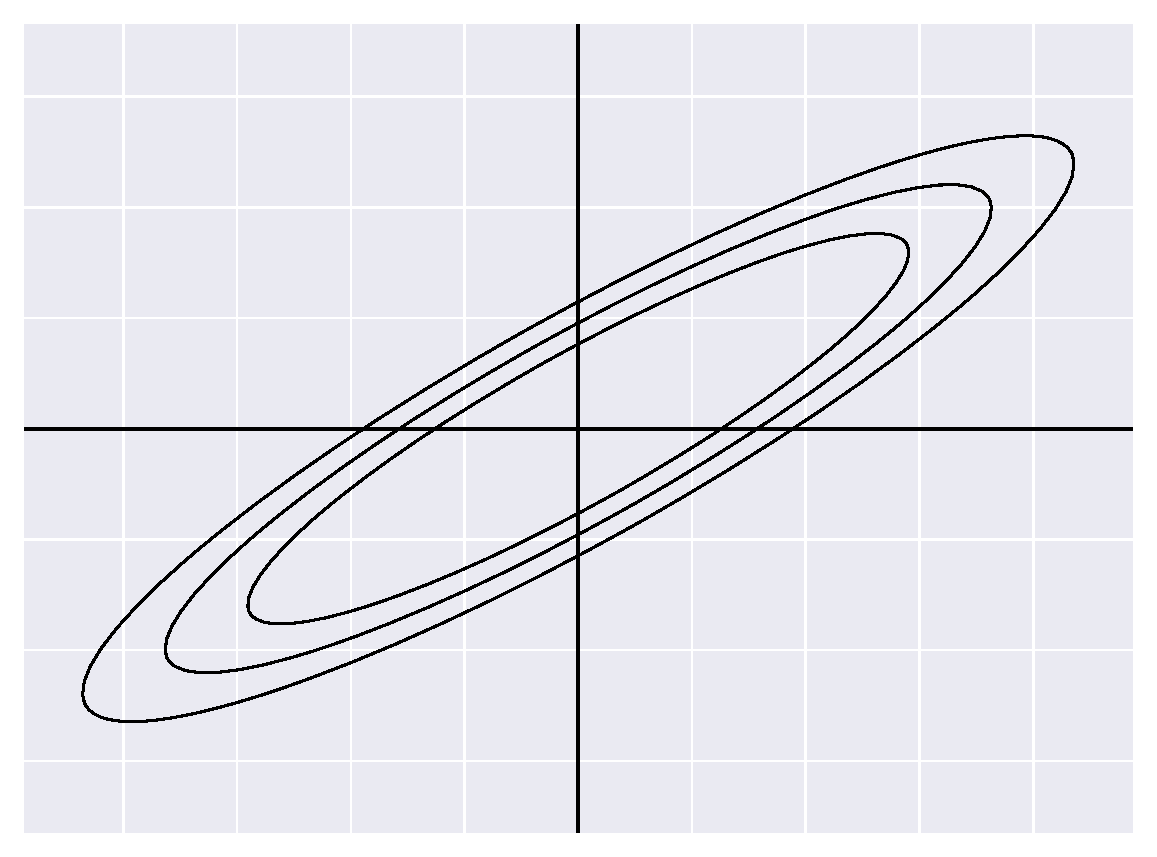
\includegraphics[height=.75\textheight]{ell1}}%
        \only<2>{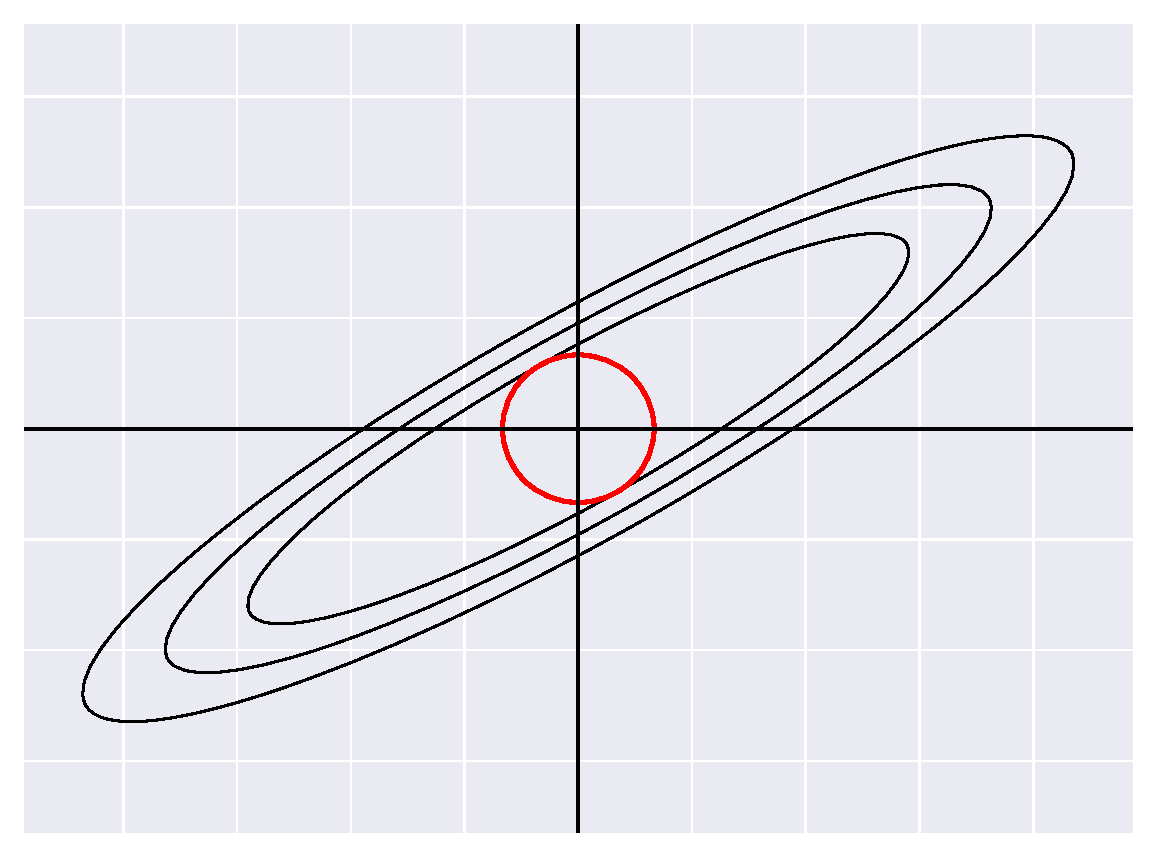
\includegraphics[height=.75\textheight]{ell2}}%
        \only<3>{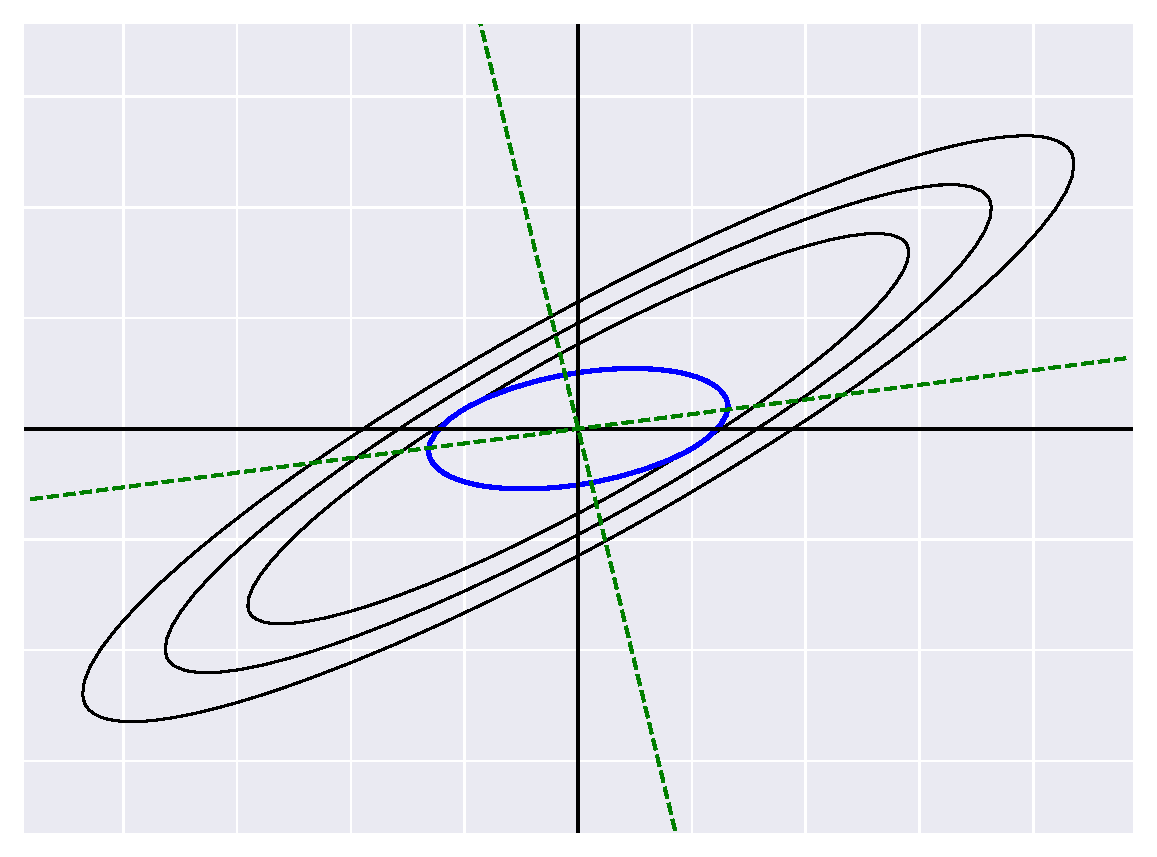
\includegraphics[height=.75\textheight]{ell3}}%
        \only<4>{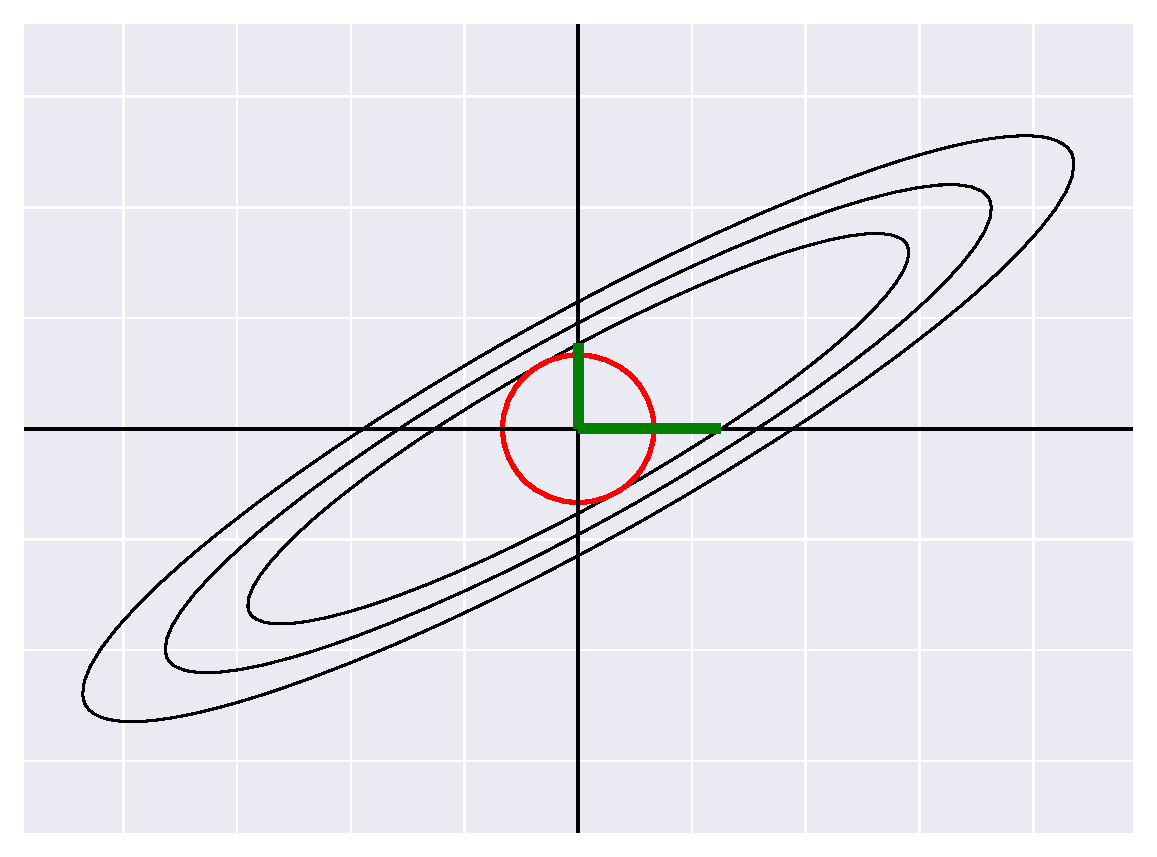
\includegraphics[height=.75\textheight]{ell4}}
    }\\
\end{frame}


\begin{frame}[t]{OISTA: Majoration-Minimization}
    For all $z$ such that $\supp(z) \subset S \doteq \supp(z^{(t)})$,
    \begin{align*}
    F_x(z) & \le f_x(z^{(t)}) + \nabla f_x(z^{(t)})^\top(z - z^{(t)})
           + \frac{\color{linkcolor} L_S}{2}\|z - z^{(t)}\|_2^2 + \lambda\|z\|_1
    \end{align*}
    with $L_S = \|D_{\cdot,S}^\top D_{\cdot,S}\|_2$.\\[1em]
    
\centering
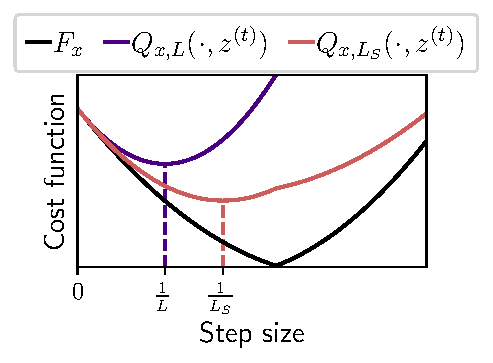
\includegraphics[width=.6\textwidth]{surrogate}\\

\end{frame}

\begin{frame}{Better step-sizes for ISTA}

    {\bf \large Oracle ISTA:\\[1em]}
    \begin{enumerate}\itemsep1em
        \item Get the Lipschitz constant $L_S$ associated with support $S = \supp(z^{(t)})$.
        \item Compute $y^{(t+1)}$ as a step of ISTA with a step-size of $1/L_S$
        \[
        y^{(t+1)} = \text{ST}\left(z^{(t)}
        - \frac{1}{L_S}D^\top(D z^{(t)} - x),
        \frac{\lambda}{L_S}\right)
        \]
        \item If $\supp(y^{t+1}) \subset S$, accept the update $z^{(t+1)} = y^{(t+1)}$.
        \item Else, $z^{(t+1)}$ is computed with step size $1/L$.
    \end{enumerate}
\end{frame}

\begin{frame}{OISTA: Performances}
    \centering
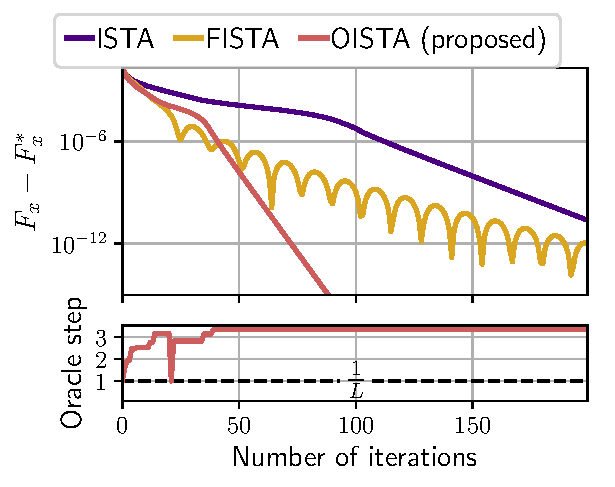
\includegraphics[width=\textwidth, trim={0 8.5em 0 0}, clip]{comparison_oista_ista}\\
\large \hskip4em Number of iterations
\end{frame}

\begin{frame}{OISTA -- Step-size}
\centering
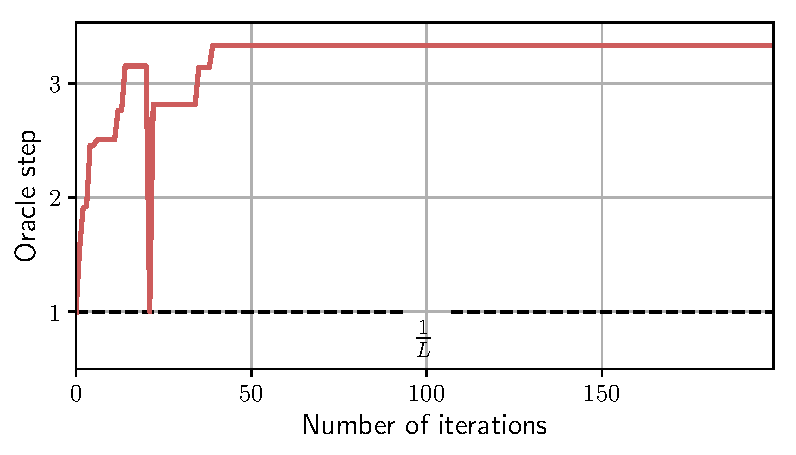
\includegraphics[width=\textwidth]{comparison_oista_ista_steps}\\
\end{frame}

\begin{frame}{OISTA -- Convergence}
    \begin{block}{Proposition 3.1: Convergence}
        When $D$ is such that the solution is unique for all $x$ and $\lambda >0$,\\
        the sequence $(z^{(t)})$ generated by the algorithm converges to $z^* =\argmin F_x~.$
        
        Further, there exists an iteration $T^*$ such that for $t\geq T^*~,$ $\supp(z^{(t)}) = \supp(z^*) \triangleq S^*$.
    \end{block}

    \begin{block}{Proposition 3.2: Convergence rate}
        For $t > T^*~,$\\
        {\centering
            $F_x(z^{(t)}) - F_x(z^*) \leq L_{S^*} \frac{\|z^{*} - z^{(T^*)}\|^2}{2(t - T^*)}~.$\\[1em]
        }
        If moreover, $\lambda_{\min}(D_{S^*}^\top D_{S^*}) = \mu^* > 0~,$ then\\[1em]
        {\centering 
            $F_x(z^{(t)}) - F_x(z^*) \leq
                (1 - \tfrac{\mu^*}{L_{S^*}})^{t - T^*}(F_x(z^{(T^*)}) - F_x(z^*))~.$\\
        }
    \end{block}
\end{frame}

\begin{frame}{OISTA -- Gaussian setting}
    \begin{block}{Acceleration quantification with Marchenko-Pastur}
        Entries in $D \in \Rset^{n \times m}$ are sampled from $\mathcal N(0, 1)$ and $S$ is sampled uniformly with $|S| = k$.
        %
        Denote $m/n \rightarrow \gamma, \enspace k /m \rightarrow \zeta \enspace ,$ with $k, m, n \rightarrow +\infty~.$ Then
        %
        \begin{equation}
        \label{eq:ratioL}
        \frac{L_S}{L} \rightarrow \left(\frac{1 + \sqrt{\zeta\gamma}}{1 + \sqrt{\gamma}} \right)^2 \enspace.
        \end{equation}
    \end{block}
    {\centering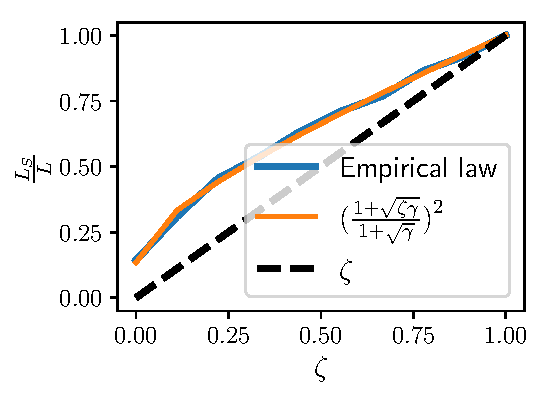
\includegraphics[width=.55\textwidth]{lip_distrib}\\}

\end{frame}

\begin{frame}{OISTA -- Limitation}
    
\begin{itemize}
    \item In practice, OISTA is not practical, as you need to compute $L_S$ at each iteration and this might be costly in time.
    \item No precomputation possible: there is an exponential number of supports $S$.
\end{itemize}

\end{frame}


\section{Using deep learning to approximate OISTA}
\parttitleframe{}

\begin{frame}[t]{Deep learning for inverse problem}
    For a direct operator $D$, the inverse problem computes
    \[
        \mathcal I_D(x) = \argmin_z \frac{1}{2}\|x - Dz\| + \lambda\|z\|_1
    \]
    Thus, the goal is not to solve {\bf one} problem but {\bf multiple} problems!\\[2em]
{\centering \large{\Large $\Rightarrow$} Can we leverage the problem's structure?\\[2em]}
\begin{itemize}\itemsep1em
    \item {\bf ISTA}: worst case algorithm, second order information is $L$.
    \item {\bf OISTA}: adaptive algorithm, second order information is $L_S$ (NP-hard).
    \item {\bf LISTA}: adaptive algorithm, use DL to learn second order information?
\end{itemize}
    
\end{frame}

\begin{frame}[t]{Learned ISTA \mycite{Gregor10}}
    Recurrence relation of ISTA define a RNN
    \begin{columns}[c]
        \column{.5\textwidth}
        \[
            z^{(t+1)} = \text{ST}\left(z^{(t)} - \frac{1}{L}D^\top(D z^{(t)} - x),
            \frac{\lambda}{L}\right)
        \]
        \column{.5\textwidth}
        {\centering
            \inputTikZ{.8}{ista_tikz.tex}\\}
    \end{columns}
    \vskip1em
    With $W_e = \frac{D\tran}{L} $ and $W_g = I - \frac{D^\top D}{L}$,
    this network is equivalent to ISTA.\\[2em]
    
    This recurrent network can be unfolded as a feed-forward network.\\[1em]
    {\centering
        \inputTikZ{.8}{lista_tikz.tex}\\}
    \vskip1em
    Let $\Phi_{\Theta^{(T)}}$ denote a network with $T$ layers parametrized with $\Theta^{(T)}$
\end{frame}


\begin{frame}[t]{LISTA -- Parametrizations}
    \setbeamercovered{transparent}
    \uncover<1>{
        {\bf General LISTA model} \mycite{Gregor10}
        \[
        z^{(t+1)} = \text{ST}\left(\textcolor{linkcolor}{\bf W_e^{(t)}}z^{(t)}
                                 + \textcolor{linkcolor}{\bf W_x^{(t)}}x,
                                   \textcolor{linkcolor}{\bf \theta^{(t)}}\right)
        \]
        The structure of $D$ is lost in the linear transform.\\[2em]
    }
    
    {\bf Coupled LISTA} \mycite{Chen2018}
    \[
    z^{(t+1)} = \text{ST}\left(z^{(t)} - \textcolor{linkcolor}{\bf\alpha^{(t)} W^{(t)}}(D z^{(t)} -x), \textcolor{linkcolor}{\bf\theta^{(t)}}\right)
    \]
    Can be seen as learning\\[1em]
    \begin{columns}[c]
        \column{.3\textwidth}
        \myitem Pre-conditionner\\
        {\centering $W^{(t)} \in \Rset^{m\times n}$\\}
        \column{.3\textwidth}
        \myitem Step-size\\
        {\centering $\alpha^{(t)} \in \Rset_+$\\}
        \column{.3\textwidth}
        \myitem Threshold\\
        {\centering $\theta^{(t)} \in \Rset_+$\\}
    \end{columns}
    \vskip1.5em
    \visible<2>{\centering {\Large $\Rightarrow$} \large Justified theoretically for (un)supervised  convergence\\}
\end{frame}


\begin{frame}{Step LISTA \mycite{Ablin2019}}

    {\bf Restricted parametrization :} 
    Only learn a step-size $\alpha^{(t)}$\\[1em]
    \[
    z^{(t+1)} = \text{ST}\left(z^{(t)}
              - \textcolor{linkcolor}{\bf\alpha^{(t)}} D^\top(D z^{(t)} -x),
              \lambda\textcolor{linkcolor}{\bf\alpha^{(t)}}\right)
    \]
    \vskip1em
    \underline{Fewer parameters:}
    $T$ instead of $( 2 + MN)T~.$\\[1em]
\begin{columns}[c]
    \column{.5\textwidth}
        \centering $\Rightarrow$ Easier to learn\\
    \column{.5\textwidth}
        \centering $\Rightarrow$ Reduced performances?\\
\end{columns}
    \vskip2em
    \underline{Goal:} Learn adapted step sizes for ISTA.\\[1em]

\end{frame}

\begin{frame}{LISTA -- Training}

    {\bf Training :}
    Given a distribution $p$ in the input space $\Rset^{n},$ the training solves
    \[
    \tilde{\Theta}^{(T)} \in \arg\min_{\Theta^{(T)}}
        \mathbb{E}_{x\sim p}[\mathcal L_x(\Phi_{\Theta^{(T)}}(x))] \enspace .
    \]
    for a given loss $\mathcal L_x~.$\\[2em]
    \strongpoint{Choice of loss $\mathcal L_x$?}
\end{frame}

\begin{frame}{LISTA -- Training}
    \centering
    \setbeamercovered{transparent}
    \setlength{\bodywd}{.9\linewidth}
    \uncover<1>{\highlight[c=black, wd=\bodywd]{
        \raggedright
        \textcolor{darkred}{\bf Supervised:}
        \normalfont a ground truth $z^*(x)$ is known
        \vskip-.5em
        \[
            \mathcal L_x(z) = \frac{1}{2}\|z - z^*(x)\|
        \]
        \vskip-.2em
        Solving the inverse problem directly.\\
     }\vskip1em
    \highlight[c=black, wd=\bodywd]{
         \raggedright
         \textcolor{darkred}{\bf Semi-supervised:}
         \normalfont the solution of the Lasso $z^*(x)$ is known
         \vskip-.5em
         \[
         \mathcal L_x(z) = \frac{1}{2}\|z - z^*(x)\|
         \]
         \vskip-.2em
         Accelerating the resolution of the Lasso.\\
    }}\vskip1em
\visible<1-2>{
    \highlight[c=black, wd=\bodywd]{
        \raggedright
        \textcolor{darkred}{\bf Unsupervised:}
        \normalfont there is no ground truth
        \vskip-.5em
        \[
        \mathcal L_x(z) = \frac{1}{2}\|x - Dz\|_2^2 + \lambda \|z\|_1
        \]
        \vskip-.2em
        Solving the Lasso directly.\\
    }}
\end{frame}

\begin{frame}[t]{Interlude -- regularization $\lambda$}
    Importance of the parameter $\lambda$
    \[
    \mathcal L_x(z) = \frac{1}{2}\|x - Dz\|_2^2 + \lambda \|z\|_1
    \]
   \[
   z^{(t+1)} = \text{ST}\left(z^{(t)}
   - \textcolor{linkcolor}{\bf\alpha^{(t)}} D^\top(D z^{(t)} -x),
   \lambda\textcolor{linkcolor}{\bf\alpha^{(t)}}\right)
   \]
   Control the distribution of $z^*(x)$ sparsity.\\[.5em]
\begin{columns}[c]
    \column{.45\textwidth}
        \begin{block}{Maximal value}
            $\lambda_{\max} = \|D^\top x\|_\infty$ is the minimal value of $\lambda$ for which
            \[
                z^*(x) = 0
            \]
        \end{block}
    \column{.45\textwidth}
    \begin{block}{Equiregularization set}
        Set in $\Rset^n$ for which $\lambda_{\max} = 1$
        \[
            \mathcal B_\infty = \{ x \in \Rset^n ~;~~ \|D^\top x\|_\infty =1\}
        \]
        \vskip1em
    \end{block}
\end{columns}

\strongpoint{Training performed with points sampled in $\mathcal B_\infty$}
   
   
\end{frame}

\begin{frame}[t]{Performances}

    {\bf Simulated data:} $m=256$ and $n=64$\\[.7em]
    \hskip6ex $D_k \sim \mathcal U(\mathcal S^{n-1})$ and $x = \frac{\widetilde x}{\|D^\top \widetilde x\|_\infty}$ with $\widetilde x_i \sim \mathcal N(0, 1)$\\[1.5em]
    {\centering
    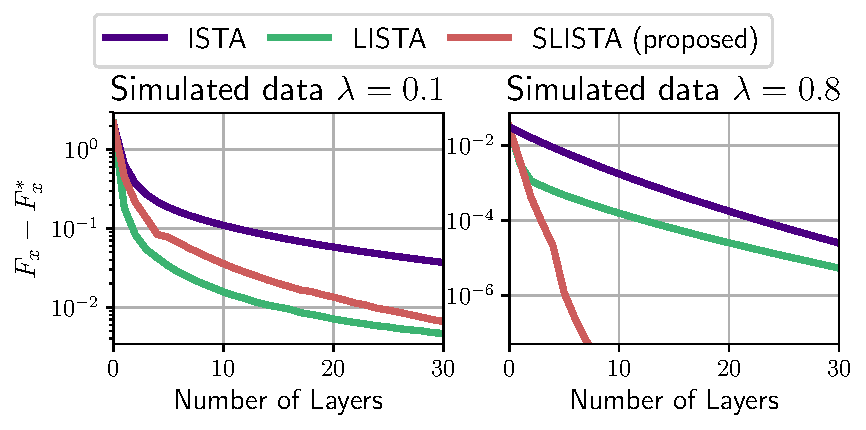
\includegraphics[width=\textwidth]{comparison_networks_simu}\\}
\end{frame}

\begin{frame}{Performance on semi-real datasets}
    
    {\bf Digits:} $8\times 8$ images \mycite{scikit-learn}\\[.7em]
    \hskip6ex $D_k $ sampled uniformly and $x = \frac{\widetilde x}{\|D^\top \widetilde x\|_\infty}$ with $\widetilde x_i \sim \mathcal N(0, 1)$\\[1.5em]
    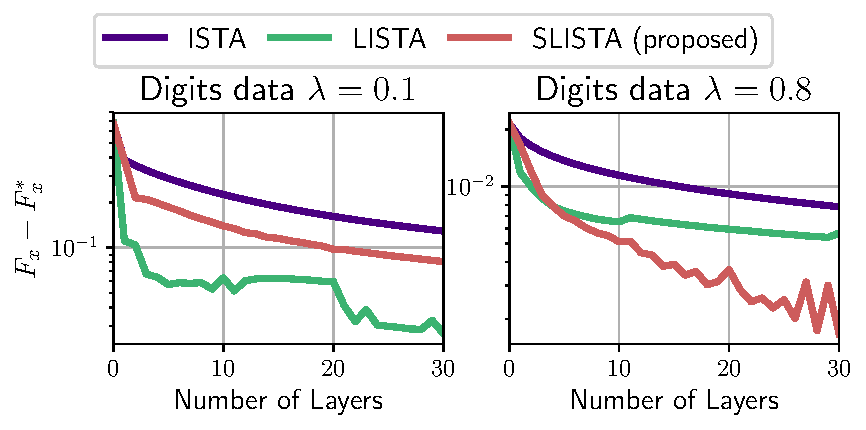
\includegraphics[width=\textwidth]{comparison_networks_images}
    
\end{frame}

\begin{frame}{Link with OISTA}
    \centering
    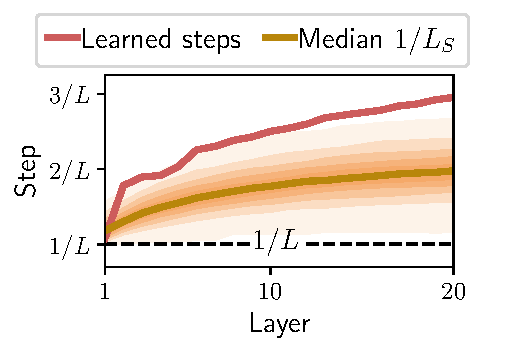
\includegraphics[width=.8\textwidth]{learned_steps}\\
    The learned step-sizes are linked to the distribution of $1/L_S$\\[2em]

\end{frame}

\section{Theoretical results}
\parttitleframe[Hold on for 2 slides!]{}

\begin{frame}{Weights coupling}
    
    We denote $\theta=(W, \alpha, \beta)$ the parameters of a given layer $\phi_{\theta}$.
    \[
    \phi_\theta(z, x) = \text{ST}\left(z - \alpha D^\top(D z -x), \lambda\alpha\right)
    \]
    \underline{Assumption 1:}\\
    \hskip3ex $D\in \Rset^{n\times m}$ is a dictionary with non-duplicated unit-normed columns.\\[1em]
    
    \begin{block}{Lemma~4.3 -- Weight coupling}
            If for all the couples $(z^*(x), x) \in \Rset^m \times \mathcal{B}_{\infty}$ such that $z^*(x)\in \argmin F_x(z)$, it holds $\phi_{\theta}(z^*(x), x) = z^*(x)$. Then, $\frac{\alpha}{\beta} W = D~.$
    \end{block}

    \vskip2em
    The solution of the Lasso is a fixed point of a given layer $\phi_{\theta}$ if and\\
    only if $\phi_{\theta}$ is equivalent to a step of ISTA with a given step-size.
\end{frame}


\begin{frame}{Asymptotic convergence of the weights}
    

\begin{block}{Theorem~4.4 -- Asymptotic convergence}  
    Consider a sequence of nested networks $\Phi_{\Theta^{(T)}}$ \emph{s.t.}\\
    $\Phi_{\Theta^{(t)}}(x) = \phi_{\theta^{(t)}}(\Phi_{\Theta^{(t + 1)}}(x), x)~.$
    Assume that
    \begin{enumerate}
        \item\label{hyp:theta_cvg} the sequence of parameters converges \ie{}
        $\theta^{(t)} \xrightarrow[t\to\infty]{} \theta^* = (W^*, \alpha^*, \beta^*) \enspace ,$
        \item\label{hyp:out_cvg} the output of the network converges toward a solution $z^*(x)$ of the Lasso uniformly over the equiregularization set $\mathcal B_\infty~,$ \ie{} $\sup_{x \in \mathcal B_\infty}\|\Phi_{\Theta^{(T)}}(x) - z^*(x)\| \xrightarrow[T \to \infty]{} 0$ \enspace.
    \end{enumerate}
    Then $\frac{\alpha^*}{\beta^*}W^* = D \enspace .$
\end{block}
\end{frame}

\begin{frame}{Numerical verification}
    \centering
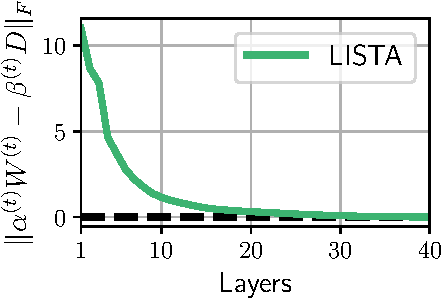
\includegraphics[width=.8\textwidth]{fro_similarity}\\[1em]
40-layers LISTA network trained on a $10 \times 20$ problem with $\lambda = 0.1$\\
{\bf The weights $W^{(t)}$ align with $D$ and $\alpha, \beta$ get coupled.}


\end{frame}

\begin{frame}{Conclusion}
    
    
\begin{itemize}\itemsep.5em
    \item Using $1/L$ as a step size is not always the fastest.
    \item Structure of the sparsity can help accelerate resolution of the Lasso.
    \item This structure can be accessed with DL.
\end{itemize}
    \vskip1em
    \underline{Take home message:}\\[.5em]
     {\centering\bf First order structure is important in optimization!\\
       No hope to learn an algorithm better than ISTA.\\
       {\hspace{0pt plus 1 filll}\normalfont\footnotesize (except for step-sizes!)}}
     
     
     \vskip1em
     \underline{Future work:}\\[.5em]
\begin{itemize}
    \item Finding a good starting point (first layer)?
    \item Adversarial cases?
\end{itemize}
\end{frame}

\begin{frame}[t]{}
    \vskip5em
    {\centering
        \usebeamercolor[fg]{title}
        \usebeamerfont{title}
        \Huge \bf Thanks!\\[2em]}
    
    \vspace{0pt plus 1 filll}
    Code available online:\\[.5em]
    
    
\includegraphics[height=.8em]{github}~\textbf{adopty} : github.com/tommoral/adopty\\[1em]
    
    Slides are on my web page:\\[.5em]
    \hskip5em\includegraphics[height=.8em]{website} tommoral.github.io
    \hskip4em 
\includegraphics[height=.8em]{twitter} @tomamoral
    
    
\end{frame}



\end{document}
